Within a framework for modeling the galaxy-galaxy and matter-galaxy power spectra $P_{\rm gg}(k)$, $P_{\rm mg}(k)$, the observed angular power spectra $C_{\ell}^{\rm gg}$, $C_{\ell}^{\rm \kappa g}$ can constrain cosmological and galaxy bias parameters. A particularly simple and interpretable model is to use the HaloFit \citep{Smith++03} fitting function for the nonlinear dark matter power spectrum, $P_{\rm mm}^{\rm HF}(k)$, and multiply by scale-independent linear biases to obtain the galaxy-galaxy and galaxy-matter power spectra,
\begin{align}
    P_{\rm gg}(k,z) &= b_{\rm gg}(z)^2 P_{\rm mm}^{\rm HF}(k,z) \\
    P_{\rm \kappa g}(k,z) &= b_{\rm \kappa g}(z) P_{\rm mm}^{\rm HF}(k,z)
\end{align}
Differences between $b_{\rm gg}$ and $b_{\rm \kappa g}$ are expected, due in large part to the stochastic contribution arising from the the fact that the galaxy field is a discrete sampling of the underlying dark matter distribution. As such, this stochastic component, which may include scale-dependent and non-Poissonian behavior, affects the galaxy-galaxy auto-spectrum and matter-galaxy cross-spectrum differently.

Using the Boltzmann code \texttt{CLASS} \citep{Blas++11} to calculate the HaloFit dark matter power spectrum for the fiducial Planck 2018 cosmology, we take the photometric $\phi(z)$ and assume a bias evolution $b_{\rm gg}(z), b_{\rm \kappa g}(z) \propto D(z)^{-1}$. We then perform weighted least squares fits of the present day biases. The results are given in Table~\ref{tab:halofit_photo}, with the fits repeated for $\ell_{\rm max} = 200, 400, 600, 800, 1000$. We find that the linear biases are unaffected by the choice of $\ell_{\rm max}$ and that the cross bias $b_{\rm \kappa g}$ is consistently lower than the galaxy bias $b_{\rm gg}$, with the latter agreeing well with DESI survey expectations and the findings of \citealt{Kitanidis++19}.  The lower-than-expected $b_{\rm \kappa g}$ could arise from choosing an incorrect fiducial cosmology (e.g.\ lowering $\Omega_m$ would reduce $b_{\rm \kappa g}$ with only a small impact on $b_{\rm gg}$; see also Hang et al., in prep).  It could also be due to the assumed bias evolution, the assumed form for $\phi(z)$ or limitations of our model.  We shall consider these next.

\begin{table}
\centering
HaloFit Model, Photo $\phi(z)$
\begin{tabular}{c|cc|cc}
\hline
$\ell_{\rm max}$ & $b_{\rm gg}$ & $\chi_{\rm gg}^2 / \text{d.o.f.}$ & $b_{\rm \kappa g}$ & $\chi_{\rm \kappa g}^2 / \text{d.o.f.}$\\
\hline
200 & $1.57 \pm 0.05$ & 0.7 / 8  & $1.27 \pm 0.07$ & 4.2 / 8 \\
400 & $1.63 \pm 0.03$ & 3.4 / 18  & $1.32 \pm 0.06$ & 8.1 / 18  \\
600 & $1.66 \pm 0.02$ & 8.4 / 28  & $1.32 \pm 0.05$ & 12.1 / 28  \\
800 & $1.67 \pm 0.02$ & 9.9 / 38  & $1.32 \pm 0.05$ & 20.9 / 38  \\
\textbf{1000} & \bm{$1.64 \pm 0.02$} & \textbf{30.4 / 48}  & \bm{$1.32 \pm 0.05$} & \textbf{26.8 / 48} \\
\hline
\end{tabular}
\caption{Fitting linear bias from the observed $C_{\ell}^{\rm gg}$, $C_{\ell}^{\rm \kappa g}$ up to different $\ell_{\rm max}$ using the HaloFit model for the nonlinear dark matter power spectrum, photometric $\phi(z)$, and the assumption $b(z) \propto D(z)^{-1}$.}
\label{tab:halofit_photo}
\end{table}

\begin{figure}
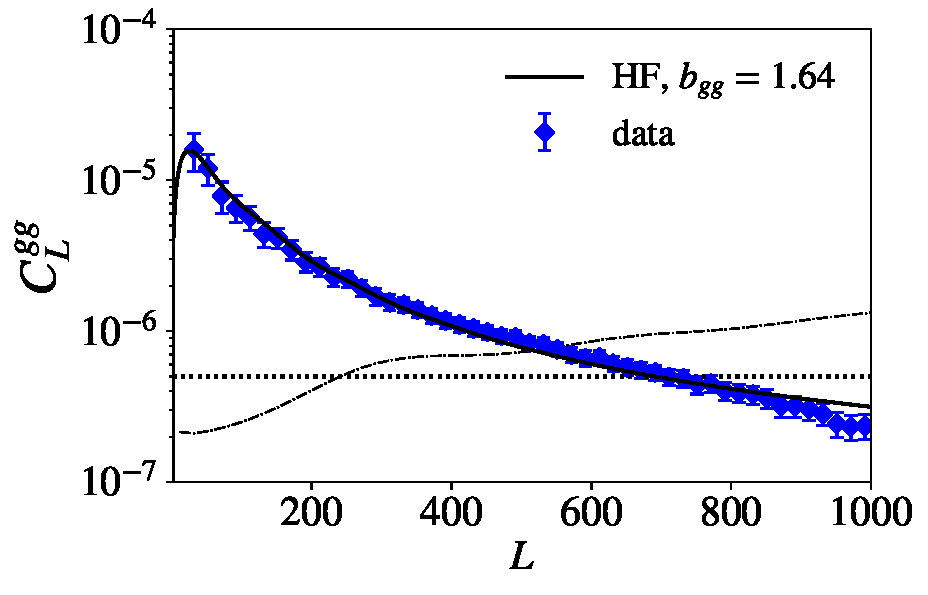
\includegraphics[width=\linewidth]{figures/cl_gg_hf.pdf}
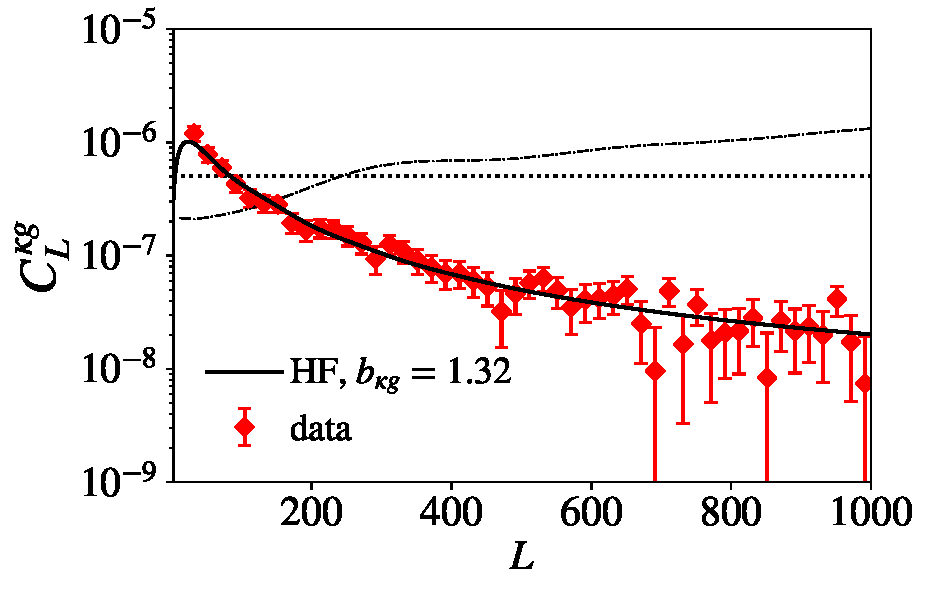
\includegraphics[width=\linewidth]{figures/cl_kg_hf.pdf}
\caption{The observed galaxy-galaxy (upper plot, blue diamonds) and galaxy-convergence (lower plot, red diamonds) angular power spectra, after subtracting noise and correcting for magnification bias. Solid lines correspond to the the theoretical predictions using a HaloFit matter power spectrum and the best fit linear biases from Table~\ref{tab:halofit_photo}. The dotted horizontal line is the galaxy shot noise floor, and the dashed black curve is the lensing noise.}
\label{fig:cl_halofit}
\end{figure}

We then repeat the same measurement using the clustering-derived $\phi(z)$ discussed in Section~\ref{sec:dndz_pipe}, again finding that the choice of $\ell_{\rm max}$ has negligible impact. The results, given in Table~\ref{tab:halofit_clustering}, show that uncertainty in the redshift distribution causes a difference in the derived galaxy bias parameters of $\sigma_{b_{\rm gg}} = 0.08$. By contrast, the cross bias is extremely stable with respect to changes in the redshift distribution, not changing at all when the redshift distribution is changed from the photometric estimate to the clustering estimate; this may be explained by the fact that the cross-spectrum only depends on one factor of $\phi(z)$ while the auto-spectrum requires $\phi^2(z)$.

Another advantage of using the clustering-based $\phi(z)$ is the ability to extract a galaxy redshift kernel with bias evolution baked in, rather than assuming a parametric form e.g. $b(z) \propto D(z)^{-1}$. As discussed in Section~\ref{sec:dndz_pipe/q}, this type of modeling allows us to constrain $b_{\rm eff} \approx b(z_{\rm eff})$ rather than the present day bias. We find the results, given in Table~\ref{tab:halofit_clustering_noevo}, to be in perfect agreement with the results of Table~\ref{tab:halofit_clustering} under the assumption $b(z) \propto D(z)^{-1}$ used in the latter, giving for instance $b_{\rm gg}= 1.56 \pm 0.01$ and $b_{\rm \kappa g}= 1.31 \pm 0.05$ for the $\ell_{\rm max} = 1000$ case. 

\begin{table}
\centering
HaloFit Model, Clustering $\phi(z)$
\begin{tabular}{c|cc|cc}
\hline
$\ell_{\rm max}$ & $b_{\rm gg}$ & $\chi_{\rm gg}^2 / \text{d.o.f.}$ & $b_{\rm \kappa g}$ & $\chi_{\rm \kappa g}^2 / \text{d.o.f.}$\\
\hline
200 & $1.50 \pm 0.05$ & 0.8 / 8  & $1.27 \pm 0.07$ & 4.0 / 8 \\
400 & $1.55 \pm 0.03$ & 3.4 / 18  & $1.32 \pm 0.06$ & 8.0 / 18  \\
600 & $1.59 \pm 0.02$ & 8.7 / 28  & $1.32 \pm 0.05$ & 11.9 / 28  \\
800 & $1.59 \pm 0.02$ & 10.2 / 38  & $1.32 \pm 0.05$ & 20.8 / 38  \\
\textbf{1000} & \bm{$1.56 \pm 0.01$} & \textbf{29.9 / 48}  & \bm{$1.32 \pm 0.05$} & \textbf{26.7 / 48} \\
\hline
\end{tabular}
\caption{Fitting linear bias from the observed $C_{\ell}^{\rm gg}$, $C_{\ell}^{\rm \kappa g}$ up to different $\ell_{\rm max}$ using the HaloFit model for the nonlinear dark matter power spectrum, clustering $\phi(z)$, and the assumption $b(z) \propto D(z)^{-1}$.}
\label{tab:halofit_clustering}
\end{table}

\begin{table}
\centering
HaloFit Model, Clustering $b(z)\phi(z)$
\begin{tabular}{c|cc|cc}
\hline
$\ell_{\rm max}$ & $b^{\rm eff}_{\rm gg}$ & $\chi_{\rm gg}^2 / \text{d.o.f.}$ & $b^{\rm eff}_{\rm \kappa g}$ & $\chi_{\rm \kappa g}^2 / \text{d.o.f.}$\\
\hline
200 & $2.14 \pm 0.07$ & 0.8 / 8  & $1.80 \pm 0.10$ & 4.0 / 8 \\
400 & $2.21 \pm 0.04$ & 3.4 / 18  & $1.89 \pm 0.08$ & 8.0 / 18  \\
600 & $2.26 \pm 0.03$ & 8.7 / 28  & $1.88 \pm 0.08$ & 12.0 / 28  \\
800 & $2.27 \pm 0.02$ & 10.2 / 38  & $1.88 \pm 0.07$ & 20.8 / 38  \\
\textbf{1000} & \bm{$2.23 \pm 0.02$} & \textbf{29.9 / 48}  & \bm{$1.88 \pm 0.07$} & \textbf{26.7 / 48} \\
\hline
\end{tabular}
\caption{Fitting effective bias $b_{\rm eff} \approx b(z_{\rm eff} = 0.68)$ from the observed $C_{\ell}^{\rm gg}$, $C_{\ell}^{\rm \kappa g}$ up to different $\ell_{\rm max}$ using the HaloFit model for the nonlinear dark matter power spectrum, clustering $b(z)\phi(z)$ (normalized), and no assumptions regarding the shape of the bias evolution.}
\label{tab:halofit_clustering_noevo}
\end{table}